\section{Filter für Bilder}

\begin{definition}[Bild]
Ein Bild ist ein \emph{zweidimensionales} Signal, also eine Funktion von $ \R^{2} \rightarrow \R $
bzw.\ von $ \Z^{2} \rightarrow \R $.
\end{definition}

\begin{definition}[Signalklassen]
Mit $ l(\Z^{2}) $ bezeichnen wir die Menge aller Signale der Form
\[
  c = \left( c(\alpha) : \alpha \in \Z^{2} \right) 
    = \left( c(\alpha_{1}, \alpha_{2}) : \alpha_{1}, \alpha_{2} \in \Z \right).
\]
Den Index $ \alpha $ nennt man auch \emph{Multiindex}.

Auch für Bilder lassen sich die Normen
\[
  \norm{c}_{p} \coloneqq \left( \sum_{\alpha \in \Z^{2}} |c(\alpha)|^{p} \right)^{1/p}, \qquad
  \norm{c}_{\infty} \coloneqq \sup_{\alpha \in \Z^{2}} |c(\alpha)|
\]
für den Fall, dass $ c \in l(\R^{2}) $, bzw.
\[
  \norm{f}_{p} \coloneqq \left( \int_{\R^{2}} |f(t)|^{p} \dif t \right)^{1/p}, \qquad
  \norm{f}_{\infty} \coloneqq \sup_{x \in \R^{2}} |f(x)|
\]
falls $ f \colon \R^{2} \rightarrow \R $, definieren. Damit sind insbesondere die Signalräume wie
$ L_{1}(\R) $, $ l_{1}(\Z) $, usw.\ für Bilder wohldefiniert.
\end{definition}

\begin{remark}[Formeln für Bilder]
Der ganze Kram, den wir in den vorherigen Abschnitten für eindimensionale Signale definiert haben,
lässt sich nun sehr leicht auf das zweidimensionale übertragen (meistens muss man bei den Formeln
einfach nur $ \R $ durch $ \R^{2} $ ersetzen und hier und da eine Variable transponieren). Seien im 
Folgenden $ f, g $ zwei Bilder (kontinuierlich modelliert).
\begin{description}
\item [Fourier-Transformation] 
  Für ein $ \xi \in \R^{2} $ ist
  \[
      \widehat{f}(\xi) 
    = \int_{\R^{2}} f(t) e^{-i \xi^{\top} t} \dif t
    = \int_{\R^{2}} f(t) e^{-i (\xi_{1}t_{1} + \xi_{2}t_{2})} \dif t
    = \int_{\R^{2}} f(t) e^{-i\xi_{1}t_{1}} e^{-i\xi_{2}t_{2}} \dif t.
  \]
\item [Faltung]
  Die Faltung von $ f $ und $ g $ ist definiert als
  \[
    f * g = \int_{\R^{2}} f(x) g(\bullet - x) \dif x.
  \]
  Auch hier gilt die sehr nützliche Identität
  \[
    (f * g)^{\wedge}(\xi) = \widehat{f}(\xi) \cdot \widehat{g}(\xi).
  \]
\item [Inverse Fourier-Transformation]
  \[
      f(x) 
    = \left( \widehat{f} \right)^{\vee}(x)
    = \frac{1}{(2\pi)^{2}} \int_{\R^{2}} \widehat{f}(t) e^{it^{\top}x} \dif t
    = \frac{1}{2\pi} \int_{\R} \frac{1}{2\pi} \int_{\R} 
        \widehat{f}(t) e^{it_{1}x_{1}} \dif t_{1} \ e^{it_{2}x_{2}} \dif t_{2}.
  \]
\item [Parseval/Plancherel]
\[
    \int_{\R^{2}} f(t)g(t) \dif t
  = \frac{1}{(2\pi)^{2}} \int_{\R^{2}} \widehat{f}(\xi) \overline{\widehat{g}(\xi)} \dif \xi
\]
und insbesondere mit $ f = g $
\[
  \norm{f}_{2} = \frac{1}{2\pi} \norm{\widehat{f}}_{2}.
\]
\item [Poisson'sche Summenformel]
\[
    \sum_{k \in \Z^{2}} f(2k\pi)
  = \frac{1}{(2\pi)^{2}} \sum_{k \in \Z^{2}} \widehat{f}(k), \qquad
    \sum_{k \in \Z^{2}} f(k)
  = \sum_{k \in \Z^{2}} \widehat{f}(2k\pi).
\]
\end{description}
Für die Beweise sei auf die entsprechenden Aufgaben auf den Übungsblättern verwiesen.
\end{remark}

\begin{remark}[LTI-Filter für Bilder]\leavevmode
\begin{itemize}
\item Verwenden wir das Kronecker-Delta als
  \[
      \delta(k) 
    = \delta_{(0,0), (k_{1}, k_{2})}
    = \delta_{0, k_{1}} \delta_{0, k_{2}}
    = \begin{cases}
        1, & k_{1}, k_{2} = 0, \\
        0, & \text{sonst},
      \end{cases}
     \qquad k = (k_{1}, k_{2}) \in \R^{2},
  \]
  dann können wir auch für Filter $ F $, die auf zweidimensionalen Signalen operieren, eine 
  Impulsantwort definieren:
  \[
    f = F\delta \in l(\Z^{2}).
  \]
\item Dementsprechend kann man, falls $ F $ ein LTI-Filter ist, die Filterung eines Bildes $ c $ 
  wieder schreiben als Faltung der Impulsantwort von $ F $ mit dem Bild:
  \[
      Fc 
    = f * c
    = \sum_{\alpha \in \Z^{2}} f(\bullet - \alpha) c(\alpha)
    = \sum_{\alpha_{1} \in \Z} \sum_{\alpha_{2} \in \Z}
        f(\bullet - (\alpha_{1}, \alpha_{2})) \ c(\alpha_{1}, \alpha_{2}).
  \]
\item Diese Formel kann man noch weiter vereinfachen, wenn $ f $ ein Tensorprodukt ist, d.h.\ falls
  \[
    f = f_{1} \otimes f_{2}, \quad f(\alpha) = f_{1}(\alpha_{1}) \cdot f_{2}(\alpha_{2})
  \]
  für $ f_{1}, f_{2} \in l(\Z) $ und $ \alpha = (\alpha_{1}, \alpha_{2}) \in \R^{2} $. Denn dann
  gilt weiter
  \begin{align*}
     f * c
  &= \sum_{\alpha_{1} \in \Z} \sum_{\alpha_{2} \in \Z}
        f(\bullet - (\alpha_{1}, \alpha_{2})) \ c(\alpha_{1}, \alpha_{2}) \\
  &= \sum_{\alpha_{1} \in \Z} \sum_{\alpha_{2} \in \Z} 
        f_{1}(\bullet_{1} - \alpha_{1}) \ f_{2}(\bullet_{2} - \alpha_{2}) \ 
        c(\alpha_{1}, \alpha_{2}) \\
  &= \sum_{\alpha_{1} \in \Z} f_{1}(\bullet_{1} - \alpha_{1})
        \sum_{\alpha_{2} \in \Z} f_{2}(\bullet_{2} - \alpha_{2}) \ c(\alpha_{1}, \alpha_{2}) \\
  &= \sum_{\alpha_{1} \in \Z} f_{1}(\bullet_{1} - \alpha_{1})
        \left( f_{2} * c(\alpha_{1}, \bullet) \right).
  \end{align*}
  Das bedeutet: Ist die Impulsantwort des LTI-Filters ein Tensorprodukt, dann erfolgt die Filterung
  eines Bildes folgendermaßen: 
  \begin{enumerate}
  \item Zuerst werden die Zeilen $ c(\alpha_{1}, \bullet) $ des Bildes für jedes feste
    $ \alpha_{1} $ mit $ f_{2} $ gefiltert. Diese Operation reduziert das Bild auf einen
    einzigen Ergebnisvektor, welchen wir als Spalte auffassen.
  \item Diese Spalte wird anschließend mit $ f_{1} $ gefiltert. Das Resultat ist dann gerade 
    $ f * c $.
  \end{enumerate}
  Als grafische Veranschaulichung sei auf Abbildung~\ref{fig:FIR-Filter-2D} verwiesen. Man kann
  sich leicht überlegen, dass die Filterung der Spalten mit $ f_{1} $ zuerst und anschließende
  Filterung der Ergebniszeile mit $ f_{2} $ zum obigen Vorgehen äquivalent ist. Wenn man das Bild um
  $ 90^{\circ} $ dreht, sollte sich ja schließlich nichts ändern, oder?
  \begin{figure}[ht]
  \centering
  \begin{tikzpicture}
  \matrix [matrix of math nodes] {
    \ddots & \vdots & \vdots & \ddots & 																		& \vdots \\
    \cdots & c(0,0) & c(0,1) & \cdots & \rightarrow f_{2} * c(0, \bullet) = & c'(0) \\
    \cdots & c(1,0) & c(1,1) & \cdots & \rightarrow f_{2} * c(1, \bullet) = & c'(1) \\
    \ddots & \vdots & \vdots & \ddots & 																		& \vdots \\
           &			  &				 & 				&																			& \downarrow \\
           &			  &				 & 				&																			& f_{1} * c' \\
           &			  &				 & 				&																			& \downarrow \\
           &			  &				 & 				&																			& f * c \\
  };
  \end{tikzpicture}
  \caption{Schematische Darstellung der Funktionsweise eines FIR-Filters für Bilder, wenn dessen
    Impulsantwort eine Tensorproduktstruktur aufweist. Zuerst wird das Bild horizontal gefiltert
    und so zu einer Spalte reduziert, welche dann vertikal gefiltert wird, um so das Endergebnis zu
    erhalten.}
  \label{fig:FIR-Filter-2D}
  \end{figure}
  
  Das ist zwar eine schöne Anschauung, aber die Darstellung von $ f $ als Tensorprodukt ist ein
  echtes Killer-Feature: Sie ermöglicht nämlich eine noch effizientere Berechnung der Filterung!
  Wir werden dies am Beispiel des Binomialfilters weiter unten kurz besprechen.
\item Auch die Transferfunktion $ \widehat{f} $ lässt sich besonders elegant schreiben, falls
  $ f = f_{1} \otimes f_{2} $:
  \begin{align*}
     \widehat{f}(\xi)
  &= \sum_{\alpha \in \Z^{2}} f(\alpha) e^{-i \alpha^{\top} \xi}
   = \sum_{\alpha_{1}, \alpha_{2} \in \Z} 
       f(\alpha_{1}, \alpha_{2}) e^{-i (\alpha_{1}\xi_{1} + \alpha_{2}\xi_{2})} \\
  &= \sum_{\alpha_{1} \in \Z} \sum_{\alpha_{2} \in \Z} 
        f_{1}(\alpha_{1}) f_{2}(\alpha_{2}) e^{-i\alpha_{1}\xi_{1}} e^{-i\alpha_{2}\xi_{2}} \\
  &= \left( \sum_{\alpha_{1} \in \Z} f_{1}(\alpha_{1}) e^{-i\alpha_{1}\xi_{1}} \right)
        \left( \sum_{\alpha_{2} \in \Z} f_{2}(\alpha_{2}) e^{-i\alpha_{2}\xi_{2}} \right) \\
  &= \widehat{f_{1}}(\xi_{1}) \cdot \widehat{f_{2}}(\xi_{2}).
  \end{align*}
  Und damit wird die Anwendung des Filters besonders einfach:
  \[
      Fc
    = \left( (Fc)^{\wedge} \right)^{\vee}
    = \left( (f * c)^{\wedge} \right)^{\vee}
    = \left( \widehat{f} \cdot \widehat{c} \right)^{\vee}
    = \left( \widehat{f_{1}} \cdot \widehat{f_{2}} \cdot \widehat{c} \right)^{\vee}.
  \]
  Die beiden Transferfunktionen $ \widehat{f_{1}} $ und $ \widehat{f_{2}} $ kann man bereits vor
  dem Anwenden des Filters berechnen, sodass wir nur noch eine schnelle Methode benötigen, um
  $ \widehat{c} $ zu bestimmen. Diese werden wir im nächsten Kapitel mit der \emph{Schnellen
  Fourier-Transformation (FFT)} kennenlernen.
\end{itemize}
\end{remark}

\begin{example}[Filter in der Bildverarbeitung]
Wir betrachten im Folgenden ein paar Beispiele für bekannte Filter in der Bildverarbeitung. Dabei
ist es meistens so, dass die Filter für Signale der Form $ \phi \colon \R^{2} \rightarrow \R $, 
also kontinuierliche Daten, konzipiert sind und später erst diskretisiert werden.
\begin{description}
\item [Mittelwertfilter] Der Mittelwertfilter $ F $ mit Impulsantwort
  \[
    f = \frac{1}{|\Omega|}\chi_{\Omega}, \qquad \Omega \subset \R^{2},
  \]
  filtert das Signal $ \phi $ mittels
  \[
      \phi(x) \mapsto (f * \phi)(x)
    = \frac{1}{|\Omega|} \int_{\R} \chi_{\Omega}(t) \phi(x - t) \dif t
    = \frac{1}{|\Omega|} \int_{\Omega} \phi(x - t) \dif t
    = \frac{1}{|\Omega|} \int_{x + \Omega} \phi(t) \dif t.
  \]
  Das heißt, er ordnet $ \phi(x) $ den Mittelwert der Menge $ x + \Omega $ zu. Um den Filter zu
  diskretisieren, setzt man einfach $ f = S_{h}\chi_{\Omega} $ und normalisiert dann, indem man 
  durch die Anzahl der in $ \Omega $ enthaltenen Abtastpunkte teilt.
  
  Ein großer Vorteil des Mittelwertfilters ist, dass er Rauschen unterdrücken kann. Dazu modelliert
  man das gemessene Signal als $ \phi(x) = \psi(x) + \epsilon(x) $, wobei $ \psi $ die eigentlichen
  Daten sind und $ \epsilon $ das (häufig als mittelwertfrei angenommene) Rauschen. Insgesamt ergibt
  sich so mit diesem Modell die Filterung
  \[
      F\phi (x)
    = \frac{1}{|\Omega|} \int_{x + \Omega} \psi(t) \dif t
        + \frac{1}{|\Omega|} \int_{x + \Omega} \epsilon(t) \dif t.
  \]
  Feine Strukturen (hohe Frequenzen) gehen so verloren, grobe Strukturen (kleine Frequenzen)
  bleiben erhalten. So gesehen verhält sich ein Mittelwertfilter wie ein Tiefpassfilter.
  
  Das Problem beim Design eines Mittelwertfilters ist die korrekte Wahl von $ \Omega $. Denn der 
  Filter angewandt auf die eigentlichen Daten $ \psi $ sollte diese weitestgehend unberührt lassen, 
  d.h.\ $ F\psi \sim \psi $. Dafür muss $ \Omega $ eine möglichst kleine Menge sein. Gleichzeitig 
  soll aber auch das Rauschen möglichst gut ausgemittelt werden, und dafür muss $ \Omega $ groß und
  \enquote{symmetrisch} genug sein.
  
  Eine andere Möglichkeit, einen Mittelwertfilter zu realisieren, ist
  \[
    f(x_{1},x_{2}) 
      = \frac{1}{2\pi\sigma^{2}} \exp\left( -\frac{x_{1}^{2} + x_{2}^{2}}{2\sigma^{2}} \right),
      \qquad \sigma > 0
  \]
  zu setzten. So steht sogar noch der freie Parameter $ \sigma $ (die Standardabweichung) zur 
  Verfügung, um das Verhalten des Filters zu spezialisieren. Für die Diskretisierung tastet man
  $ f\chi_{[-N,N]^{2}} $ für ein $ N \in \N $ ab. Die charakteristische Funktion wird benötigt, um 
  einen FIR-Filter zu erhalten, denn der Gaußkern besitzt ja unendlichen Träger. Diese 
  Diskretisierung führt uns sogleich zum nächsten Filter.
\item [Binomialfilter]
  Die Binomalfilter sind spezielle Mittelwertfilter, denen wir in einem eigenen Punkt 
  Aufmerksamkeit widmen wollen, und das diskrete Gegenstück zum oben erwähnten Gaußkern. Deren 
  Impulsantwort ist gegeben durch
  \[
      f(j,k)
    = \frac{1}{2^{m + n}} \binom{m}{j} \binom{n}{k}
    = \left( \frac{1}{2^{m}} \binom{m}{j} \right) \left( \frac{1}{2^{n}} \binom{n}{k} \right),
      \qquad 0, \ldots, m, \quad 0, \ldots, n.
  \]
  Wie man sieht, besitzt die Impulsantwort Tensorproduktstruktur. $ f $ lässt sich auch 
  als Matrix darstellen, wenn man $ j $ als Zeile und $ k $ als Spalte auffasst. Geschickt ist es, 
  $ m $ und $ n $ als gerade zahlen zu wählen, denn dann lässt sich die Matrix sogar zentrieren. Um 
  etwas Terminologie aus der Informatik zu verwenden: Man erhält so einen $ m \cdot n $-%
  Punkt-Stencil, der sukzessive über das Bild geschoben wird (mathemat.\ Faltung). Beispielsweise 
  erhält man für $ m,n = 2 $
  \[
      \frac{1}{4} \begin{pmatrix} 1 \\ \mathbf{2} \\ 1 \end{pmatrix} *
        \frac{1}{4} \begin{pmatrix} 1 & \mathbf{2} & 1 \end{pmatrix}
    = \frac{1}{16} \begin{pmatrix}
        1 & 2 & 1 \\
        2 & \mathbf{4} & 2 \\
        1 & 2 & 1
      \end{pmatrix}
  \]
  und für $ m,n=4 $
  \[
      \frac{1}{16} \begin{pmatrix} 1 \\ 4 \\ \mathbf{6} \\ 4 \\ 1 \end{pmatrix} *
        \frac{1}{16} \begin{pmatrix} 1 & 4 & \mathbf{6} & 4 & 1 \end{pmatrix}
    = \frac{1}{256} \begin{pmatrix}
        1 &  4 & 6  & 4  & 1 \\
        4 & 16 & 24 & 16 & 4 \\
        6 & 24 & \mathbf{36} & 24 & 6 \\
        4 & 16 & 24 & 16 & 4 \\
        1 &  4 &  6 &  4 & 1
      \end{pmatrix}.
  \]
  Der fett gedruckte Wert bezeichnet dabei jeweils die aktuelle Zelle des Stencils. Je größer nun 
  die Werte für $ m $ und $ n $ gewählt, werden, desto mehr benachbarte Zellen werden für die
  Berechnung hinzugezogen und umso stärker wird das Bild dadurch geglättet.
  
  Mittlerweile sollte auch aufgefallen sein, dass die Implementierung des Filters über die Faltung
  des $ m $-Punkt- mit dem $ n $-Punkt-Stencils um Größenordnungen effizienter ist als der
  $ m \cdot n $-Punkt-Stencil. Denn im ersten Fall werden lediglich $ \mathcal{O}(m + n) $ 
  Speicherzugriffe benötigt (linearer Anstieg), wohingegen im zweiten Fall 
  $ \mathcal{O}(m \cdot n) $ Speicherzugriffe fällig sind (quadratischer Anstieg). Auch die Zahl
  der auszuführenden Operationen (Addition, Multiplikation) wird so verringert. Dieser 
  Performance-Unterschied wird mit wachsenden $ n, m $ immer deutlicher. Genau hierin liegt der 
  Vorteil, wenn man es schafft, die Impulsantwort als Tensorprodukt darzustellen!
  
  Übrigens ist $ 2^{m + n} $ gerade die Summe aller Einträge in der Matrix, denn es gilt
  \begin{align*}
      \sum_{j = 0}^{m} \sum_{k = 0}^{n} \binom{m}{j} \binom{n}{k}
   &= \left( \sum_{j = 0}^{m} \binom{m}{j} \right) \left( \sum_{k = 0}^{n} \binom{n}{k} \right)
    = \left( \sum_{j = 0}^{m} \binom{m}{j} 1^{m} 1^{m - j} \right) 
        \left( \sum_{k = 0}^{n} \binom{n}{k} 1^{n} 1^{n - k} \right) \\
   &= (1 + 1)^{m} (1 + 1)^{n}
    = 2^{m} 2^{n}
    = 2^{m + n},
  \end{align*}
  sodass wir es wirklich mit einem Mittelwertfilter zu tun haben!
  
  Abbildung~\ref{fig:binom} veranschaulicht die Wirkung des Binomialfilters an einem kleinen
  Beispiel.
  \begin{figure}[ht]
  \centering
  \begin{minipage}{0.4\textwidth}
    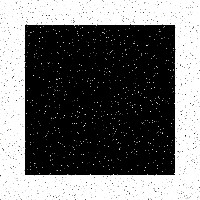
\includegraphics[width=0.7\linewidth]{Bilder/noise}
  \end{minipage}
  \begin{minipage}{0.4\textwidth}
    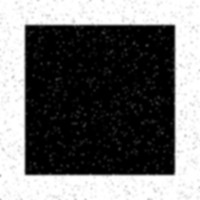
\includegraphics[width=0.7\linewidth]{Bilder/noise_binom}
  \end{minipage}
  \caption{Links: Ein ziemlich verrauschtes Bild eines Quadrats. Rechts: Anwendung des
    Binomialfilters auf das Bild. Es wurde die oben gezeigte Faltungs-Matrix für $ m,n = 4 $ 
    verwendet. Man erkennt, dass das Bild zwar deutlich entrauscht wurde, dafür sind die scharfen
    Kanten um Einiges verschwommener.}
  \label{fig:binom}
  \end{figure}
\item [Gradientenfilter]
  Der Gradientenfilter verwendet, wie der Name schon erahnen lässt, den Gradienten unseres
  Signals $ \phi $. Allgemein ist der Gradient einer Funktion $ \phi $ definiert als
  \[
    \nabla \phi(x,y) = \begin{pmatrix}
    \dpd{\phi}{x}(x,y) \\[1em]
    \dpd{\phi}{y}(x,y)
    \end{pmatrix}.
  \]
  Anschaulich: Wir bilden die partiellen Ableitungen zu $ \phi $ und stecken diese in einen Vektor 
  (den Gradienten). Dieser zeigt dann in diejenige Richtung, in der $ \phi $ an der Stelle $ (x,y) $
  am stärksten steigt oder fällt. So können wir Konturen und Kanten im Bild erkennen. Denn eine 
  Kontur findet sich ja dort, wo der (Farb-)Unterschied zwischen benachbarten Pixeln groß ist und
  damit die Steigung groß ist.
  
  Den Gradienten für ein diskretes Signal $ c $ können wir definieren über den
  Differenzen-Quotienten als
  \[
      \nabla c(x,y)
    = \begin{pmatrix}
        \nabla_{x} c(x,y) \\
        \nabla_{y} c(x,y)
      \end{pmatrix}
    = \begin{pmatrix}
        c(x + 1, y) - c(x, y) \\
        c(x, y + 1) - c(x, y)
      \end{pmatrix}.
  \]
  Die Impulsantwort lässt sich darstellen als Matrix von Vektoren
  \[
      \left( \nabla \delta(x,y) \right)_{-1 \leq x,y \leq 1}
    = \begin{pmatrix}
        \begin{pmatrix} 0 \\ 0 \end{pmatrix} &
        \begin{pmatrix} 1 \\ 0 \end{pmatrix} & 
        \begin{pmatrix} 0 \\ 0 \end{pmatrix} \\[1em]
        \begin{pmatrix} 0 \\ 1 \end{pmatrix} &
        \begin{pmatrix} \mathbf{-1} \\ \mathbf{-1} \end{pmatrix} &
        \begin{pmatrix} 0 \\ 0 \end{pmatrix} \\[1em]
        \begin{pmatrix} 0 \\ 0 \end{pmatrix} &
        \begin{pmatrix} 0 \\ 0 \end{pmatrix} &
        \begin{pmatrix} 0 \\ 0 \end{pmatrix}
      \end{pmatrix},
  \]
  beziehungsweise
  \[
      \left( \nabla_{x} \delta(x,y) \right)_{-1 \leq x,y \leq 1}
    = \begin{pmatrix}
        0 & 1 & 0 \\
        0 & \mathbf{-1} & 0 \\
        0 & 0 & 0
      \end{pmatrix}, \qquad
      \left( \nabla_{y} \delta(x,y) \right)_{-1 \leq x,y \leq 1}
    = \begin{pmatrix}
        0 & 0 & 0 \\
        1 & \mathbf{-1} & 0 \\
        0 & 0 & 0
      \end{pmatrix}.
  \]

  Leider sind solche Gradientenverfahren inhärent empfindlich gegen Rauschen. Und je genauer man 
  das Signal abtastet, umso mehr wird das Rauschen durch den Gradientenfilter noch verstärkt. Daher
  kombiniert man den Gradienten mit einem Mittelwertfilter, z.B. den Mittelungsoperator
  \[
    m \coloneqq
    \frac{1}{9} \begin{pmatrix}
      1 & 1 & 1 \\
      1 & \mathbf{1} & 1 \\
      1 & 1 & 1
    \end{pmatrix}.
  \]
  Die Faltungen $ m * \nabla_{x} $ und $ m * \nabla_{y} $ ergeben dann die Matrizen
  \[
      m * \nabla_{x}
    = \frac{1}{9} \begin{pmatrix}
        1 & 1 & 1 \\
        0 & 0 & 0 \\
        0 & \mathbf{0} & 0 \\
        -1 & -1 & -1
      \end{pmatrix}, \qquad
      m * \nabla_{y}
    = \frac{1}{9} \begin{pmatrix}
        1 & 0 & 0 & -1 \\
        1 & \mathbf{0} & 0 & -1 \\
        1 & 0 & 0 & -1
      \end{pmatrix}.
  \]
  Die linke Matrix erkennt dabei Kanten, die in $ x $-Richtung verlaufen, und die rechte Matrix
  entsprechend Kanten in $ y $-Richtung. Siehe hierfür Abbildung~\ref{fig:Gradient}.
  \begin{figure}[ht]
  \centering
    \begin{minipage}{0.3\textwidth}
    
\includegraphics[width=\textwidth]{Bilder/Gradient}
    \end{minipage}
    \hfill
    \begin{minipage}{0.3\textwidth}
    
\includegraphics[width=\textwidth]{Bilder/Gradient_x}
    \end{minipage}
    \hfill
    \begin{minipage}{0.3\textwidth}
    
\includegraphics[width=\textwidth]{Bilder/Gradient_y}
    \end{minipage}
  \caption{Wirkung des Gradientenfilters. Links: Unser Testbild, welches nur aus einem schwarzen 
    Quadrat besteht. Mitte: Anwendung von $ m * \nabla_{x} $ findet alle Kanten in $ x $-
    Richtung. Rechts: Anwendung von $ m * \nabla_{y} $ findet alle Kanten in $ y $-Richtung.
    Bedingt durch die unterschiedliche Gewichtung (Einträge $ 1 $ und $ -1 $ in den Matrizen)
    werden die Kanten entweder weiß oder schwarz gezeichnet.}
  \label{fig:Gradient}
  \end{figure}
  Um Kanten in beide Richtungen gleichzeitig zu finden, kann man beispielsweise beide Matrizen über 
  die $ 1 $-Norm des geglätteten Gradienten kombinieren:
  \[
    \norm{m * \nabla c}_{1} = |m * \nabla_{x} c| + |m * \nabla_{y} c|.
  \]
  Oder man verwendet den Laplace-Filter, welchen wir als Nächstes behandeln.
\item [Laplace-Filter] Der Laplace-Filter verwendet den Laplace-Operator
  \[
      \Delta \phi(x,y) 
    = \left\langle \nabla \phi(x,y), \nabla \phi(x,y) \right\rangle
    = \dpd[2]{\phi}{x}(x,y) + \dpd[2]{\phi}{y}(x,y),
  \]
  welcher das Skalarprodukt des Gradienten eines kontinuierlichen Signals $ \phi $ mit sich selbst, 
  also die Summe der zweiten Partiellen Ableitungen bildet. Die Idee dabei ist, dass die zweiten
  Ableitungen lokale Extrema angeben. Am Beispiel von Bildern sind dies genau diejenigen Stellen,
  an denen es die gravierendsten (Farb-)Unterschiede zwischen benachbarten Pixeln gibt. Und dies
  sind häufig Kanten.
  
  Diskretisierungen des Laplace-Operators sind beispielsweise
  \[
    \begin{pmatrix}
      0 & 1 & 0 \\
      1 & \mathbf{-4} & 1 \\
      0 & 1 & 0
    \end{pmatrix}, \qquad
    \begin{pmatrix}
      1 & 1 & 1 \\
      1 & \mathbf{-8} & 1 \\
      1 & 1 & 1
    \end{pmatrix}.
  \]
  
  Wie die Gradientenfilter auch ist der Laplace-Operator sehr rauschempfindlich, sodass es sich
  wieder empfiehlt, diesen mit einem Glättungsfilter zu kombinieren. Gut geeignet ist z.B.\ der
  Medianfilter.
\item [Medianfilter] Der Medianfilter
  \[
    Mc(j) = \Median\{ c(k) : k \in j + \Omega \}, \qquad \Omega \subset \Z^{2}
  \]
  sortiert alle Werte $ c(j + \Omega) $ der Größe nach und wählt daraus den Wert in mittlerer
  Position aus. Da er Bilder entrauscht, Kanten erhält und von wenigen Ausreißern unberührt
  arbeitet, wird er häufig zur in Kombination mit anderen Filtern, z.B.\ zur Kantendetektion, 
  eingesetzt. Allerdings ist der Medianfilter kein linearer Operator und besitzt wegen des 
  Sortierens einen vergleichsweise hohen Rechenaufwand von mindestens $ \mathcal{O}(n \log n) $.
\end{description}
\end{example}